\subsubsection{Electronic design}
In this project, the user interface is implemented in the form of an android application. Commands are communicated to a microcontroller via a serial connection with a Bluetooth module. The microcontroller does all of the calculations and performs the necessary algorithms to determine what should be done with which servo and then communicates this to the relevant servo motor. The algorithm for movement also takes some inputs from the microcontroller into account.\\

The electronics to be implemented for this project therefore includes the following list. Each item is discussed separately below.
\begin{itemize}
\item Power regulation and supply.
\item Support electronics for the microcontroller.
\item Digital input signal conditioning.
\item Bluetooth module interfacing.
\item Digital output driving where applicable.
\item Servo power control switch
\end{itemize}

Power regulation and supply for the project can be divided into two parts. The first of these is the low voltage, low power part that supplies the microcontroller, Bluetooth module and support electronics. The second part is the higher voltage, high power part that supplies power exclusively to the servo motors. Both these supplies will be powered by Li-Ion 18650 cells because of their high power density. The nominal voltage of these cells are $3.7V$. The low voltage, low power supply can easily be powered from a single cell making use of a low dropout (LDO) linear regulator to provide the $3.3V$ rail required. A linear voltage regulator is not suited for the high power application, mainly for two reasons. The first of the two is that these regulators are rarely rated for use above $1.5A$. The second is that a linear regulator dissipates power in itself as heat in order to regulate voltage. This means that the voltage drop formed over the device to bring the output voltage down is dissipated in the device. The power dissipated can be quantified by

\begin{align}
P &= V\times I\\
&= (V_{in}-V_{out})\times I
\end{align}

This is fine for low current applications but sufficient cooling quickly becomes a problem at currents in the Ampere range.
A better solution for regulation at high power is making use of a step-down DC-DC converter. The efficiency of this topology is much greater than for linear regulators. Most are in excess of $90\%$ if operated within the design limits. Since DC-DC converters can become very complex and it is far outside the scope of this project, a complete off-the-shelf module was implemented instead of designing and building one from first principles. Figure \ref{fig:PowerSupply} shows the power supply layout for the robot.

\begin{figure}[H]
\centering
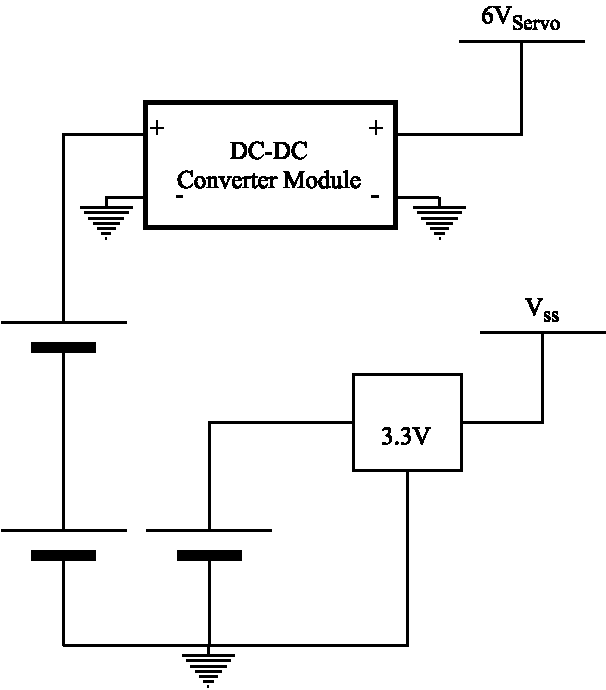
\includegraphics[scale = 1]{pics/PowerSupply.pdf}
\caption{Diagram showing the power supply layout for the robot}
\label{fig:PowerSupply}
\end{figure}

The support electronics for the microcontroller includes everything necessary for it to be able to start after power up and function normally. The application note provided by the manufacturer has detailed instructions and schematics on this and it was implemented as recommended for this project. This includes ceramic capacitors on all of the power supply pins, electrolytic capacitors on the power rails, a high frequency crystal oscillator, timing capacitors, a reset switch, various pull-up and pull-down resistors and a selector for pulling the BOOT pin high or low. More details on this can be fond in the technical documentation section of the report.

\subsubsection{Electronic implementation}